\chapter{Mappa e funzionalità}
% \section{Mappa e sue funzionalità}
La pagina della mappa è stata la sezione dell'applicazione più difficile da
implementare, perchè al suo interno risiedono numerosi servizi e funzioni che
hanno richiesto diverso tempo per essere sviluppati e inoltre è stato necessario
documentarsi per capire come utilizzare le API che la pagina utilizza.

\section{Scelta del servizio API}
% \subsection{Scelta del servizio API}
In un primo momento si è pensato di utilizzare il servizio mappe di Google Maps
che, oltre ad essere uno dei più efficienti e meglio documentati, è anche
implementabile facilmente. Il problema è nato nel momento in cui Google ha
deciso di cambiare le proprie politiche di utilizzo delle API verso la fine del
2018. Prima di quel momento, sotto a un certo numero di richieste al servizio di
geolocalizzazione il programmatore poteva usare liberamente il codice e senza
necessità di registrazione, ma in seguito l'azienda di Mountain View ha deciso
che chiunque volesse utilizzare il proprio servizio mappe dovesse prima
registrare un proprio account ed inserire una carta di credito che eventualmente
pagasse mensilmente le risorse di cui si è fatto uso. Questo scenario ha portato
a prendere in cosiderazione altri gestori di mappe. La scelta è ricaduta su
MapBox, azienda emergente nel proprio campo. Il servizio era gratuito e permetteva
un agevole utilizzo senza registrazione ma il problema era formato
dall'implementazione vera e propria. Al contrario di Google, non esiste un
pacchetto software che implementi il codice MapBox e quindi era necessario fare
uso di richieste http tramite valori codificati all'interno di lunghi url.
Inoltre la fluidità della mappa non rispettava le direttive del committente
dott. Marco Aceti, spesso a seguito di un rapido movimento delle dita per
spostarsi in un'altra zona della mappa la schermata rimaneva per qualche secondo
completamente grigia, rendendo l'esperienza di utilizzo sicuramente peggiore.
Nel seguito, tra Gennaio e Febbraio 2019 è stata rilasciata la prima versione
ufficiale di Flutter (versione 1.0.0) e tra le tante novità spiccava la presenza
di un widget particolare, chiamato \textit{GoogleMap}. Semplificando notevolmente
l'utilizzo delle mappe, tale widget presenta ottime prestazioni e facilità di
implementazione. Si è quindi deciso di dedicare del tempo nell'apprendere ogni
aspetto delle politiche di utilizzo delle API di Google, capendo quindi che,
facendo un numero di richieste minore di una soglia stabilita, non è necessario
pagare nulla, anche se si è registrata una carta di credito. Quindi la scelta è
ricaduta sulle API di Google e si è importato nel progetto il pacchetto
\verb|googlemap|.

\section{MapPage}
% \subsection{MapPage}
Dopo che l'utente ha eseguito correttamente la procedura di login o ha aperto
l'applicazione in caso di autoidentificazione con mantenimento dello stato della
registrazione, viene mostrata la MapPage. \\
In alto è presente un'AppBar che 
mostra il titolo eBike-Recharge, in basso è presente una TabBar che permette di
navigare tra le pagine dell'app. Tra le due, a tutto schermo, viene mostrata la
mappa con al centro la posizione attuale dell'utente. Quest'ultima può essere di
diversi tipi a seconda delle preferenze indicate nella pagina profilo
dell'utilizzatore. In particolare si può scegliere tra \textit{Normale}, cioè la
classica modalità di visualizzazione di mappe che viene mostrata di default
sull'app Google Maps, \textit{Rilievo}, dove è presente l'altitudine delle
montagne indicata con diversi colori in base all'altezza, mancando però
di indicare i nomi di edifici importanti, negozi o imprese, \textit{Satellite},
che mostra con una serie di foto satellitari i luoghi indicati dall'alto, in
modo da vedere realmente il percorso che si deve intraprendere
per raggiungere la propria destinazione, e \textit{Ibrida}, che può essere
considerata l'unione di Satellitare e Normale, poichè oltre a presentare
l'altitudine mostra anche i nomi dei luoghi di maggior importanza della zona
visualizzata.

\begin{figure}[h!]
    \centering
    \begin{subfigure}{0.33\linewidth}
        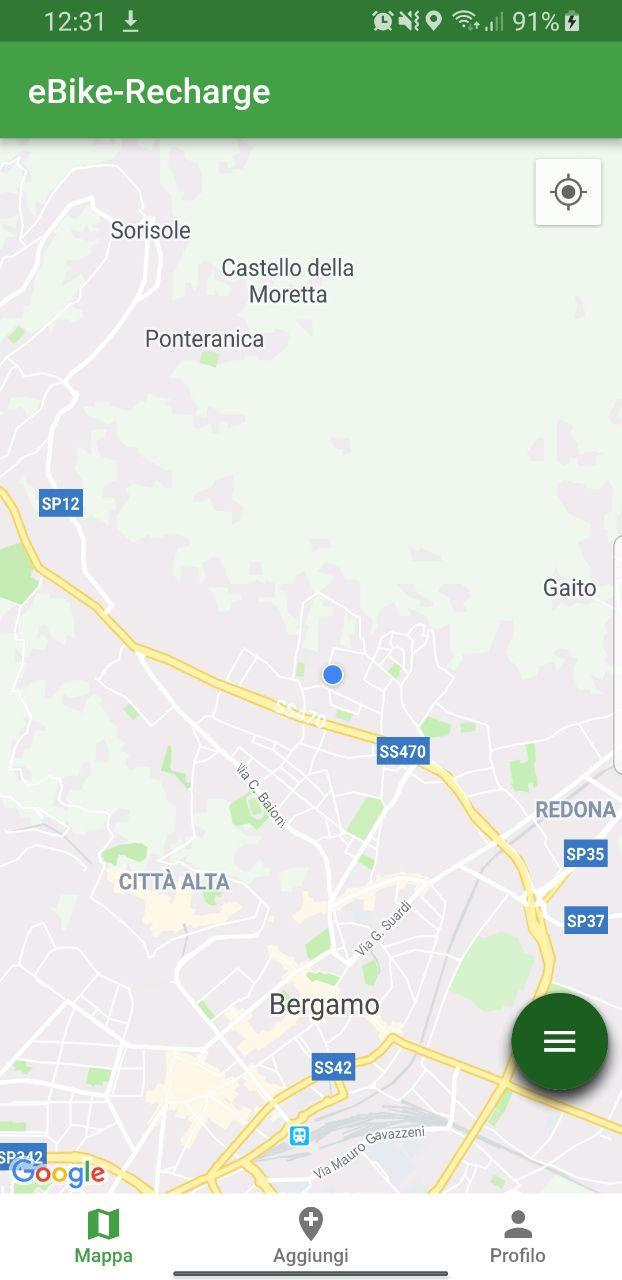
\includegraphics[width=\linewidth, height=9cm]{MapNormale.jpg}
        \caption{Normale}
    \end{subfigure}
    \begin{subfigure}{0.33\linewidth}
        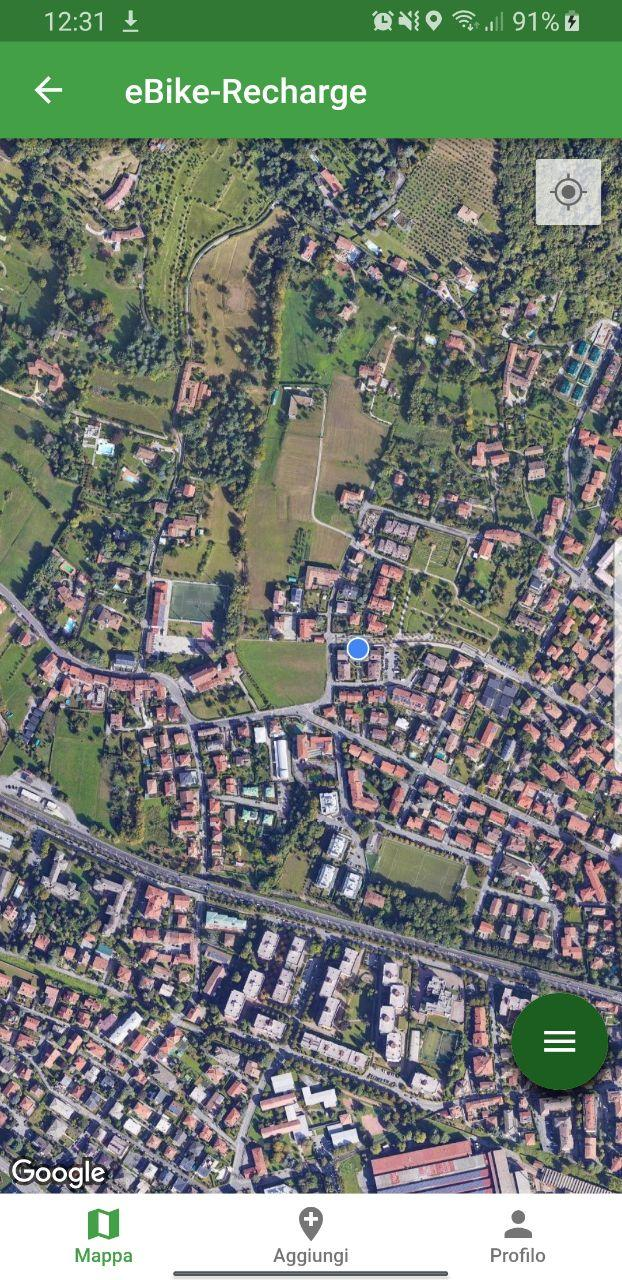
\includegraphics[width=\linewidth, height=9cm]{MapSatellite.jpg}
        \caption{Satellite}
    \end{subfigure}
    \begin{subfigure}{0.33\linewidth}
        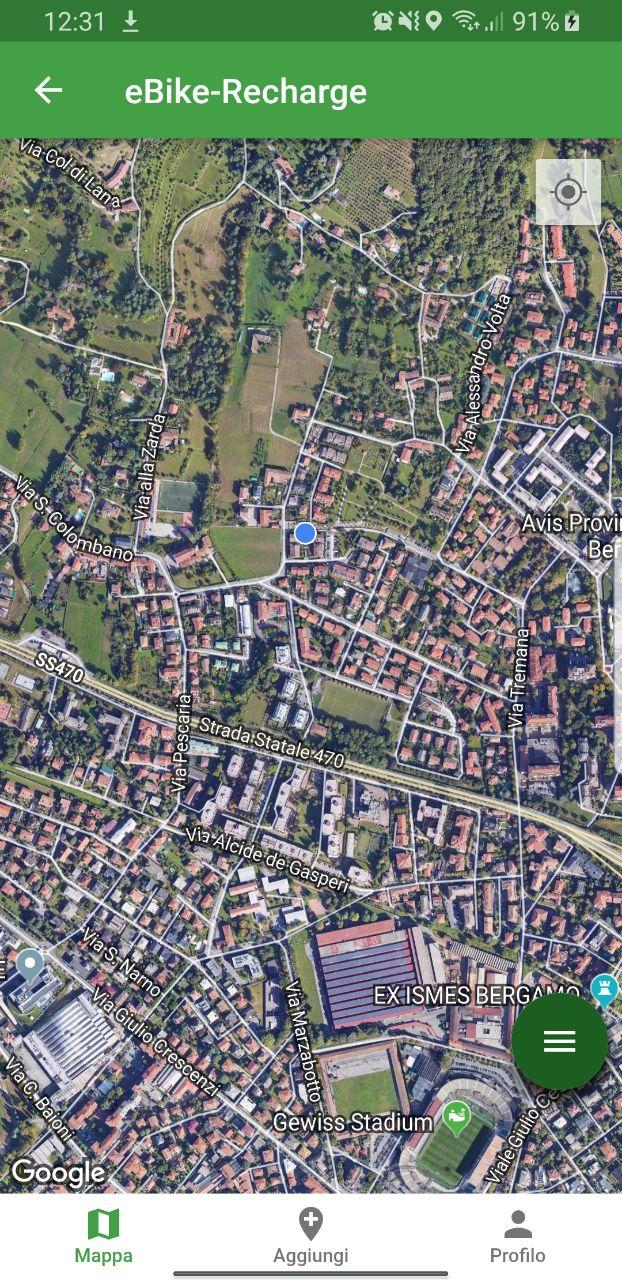
\includegraphics[width=\linewidth, height=9cm]{MapIbrida.jpg}
        \caption{Ibrida}
    \end{subfigure}
    \begin{subfigure}{0.33\linewidth}
        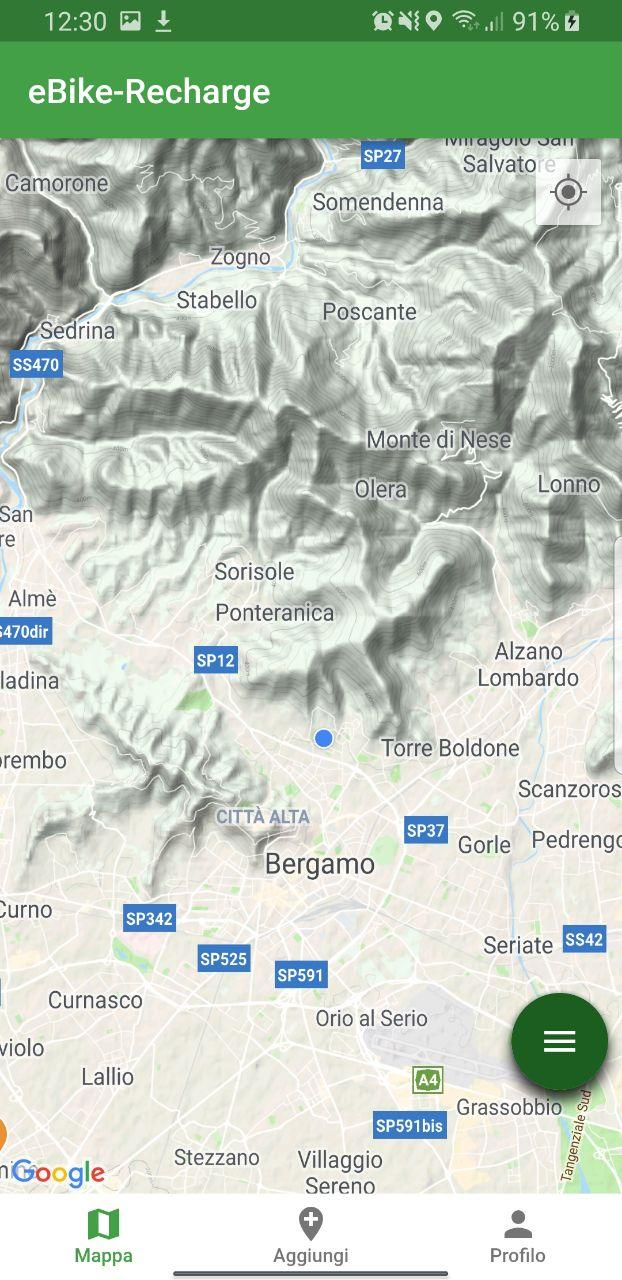
\includegraphics[width=\linewidth, height=9cm]{MapRilievo.jpg}
        \caption{Rilievo}
    \end{subfigure}
    \caption{I quattro tipi di mappa selezionabili nella pagina profilo}
    \label{TipoMappa}
\end{figure} 

Grazie al pacchetto \textit{googlemap} di flutter si è riusciti a implementare un oggetto
GoogleMap (che verrà descritto in un successivo paragrafo) con cui è molto
facile interagire. In particolare, l'utente può aumentare o diminuire lo zoom
della mappa mediante gesture e
può spostarsi in diverse zona semplicemente trascinando verso la direzione
desiderata. Con una buona o anche solo media connessione internet i tempi di
latenza sono pressochè nulli, così che non si riesca a vedere i riquadri grigi
che il widget crea nel momento in cui si cambia direzione e che dovranno essere
riempiti con le nuove località. Questi ultimi sono pienamente visibili nel
momento in cui non si disponga di una connessione adeguata, condizione che si
verifica sempre più di rado negli ultimi tempi. 


\section{Funzionalità}
% \subsection{Funzionalità}
Nelle immagini precedenti viene inoltre mostrato un pulsante nella parte inferiore
dello schermo verso destra. Se premuto (figura \ref{4puls}), quest'ultimo mostra una serie di
pulsanti con diverse funzionalità.
\begin{figure}[!h]
    \centering
    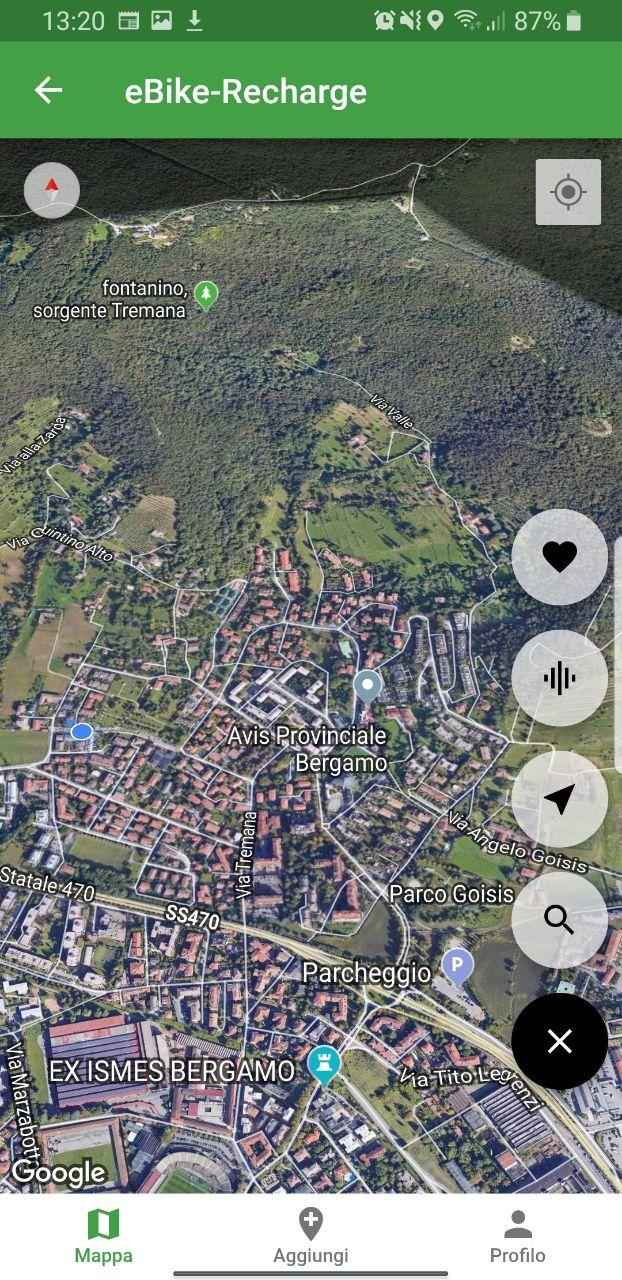
\includegraphics[width=7cm]{MapFun.jpg}
    \caption{Premuto il pulsante, vengono mostrati i 4 FloatingActionButton e il quinto (con la X) per tornare indietro}
    \label{4puls}
\end{figure}
Il primo è un'icona a forma di cuore e,
interagendo con esso, viene mostrato un BottomSheet (spiegato nel secondo
capitolo, Flutter) che mostra una Card (una piccola scheda con titolo e icona)
con le stazioni di ricarica preferite dall'utente. Per esprimere la propria
preferenza per una stazione è necessario entrare nella scheda di quest'ultima e
selezionare l'icona a forma di cuore presente in alto a destra. \\
Il secondo pulsante ha la funzione di filtro e al tempo stesso di legenda.
Premendolo, viene mostrata a schermo una AlertDialog (fig. \ref{filtro}) che indica quali
tipologie di stazioni si possono cercare. Sulla destra sono presenti dei Button
di tipo check (che possono essere True o False): se si vede la casella spuntata
allora si vedra la relativa tipologia sulla mappa, se tale casella è vuota
allora la mappa verrà filtrata e non sarà possibile cercare tutte le stazioni di
quel tipo. \\
Il terzo pulsante mostra un'icona con la classica freccia indicante la
navigazione e, se premuto, fa apparire un BottomSheet con Card contenente le
dieci stazioni più vicine alla posizione attuale dell'utente. Come per tutte le
Card anche nelle altre funzionalità, è possibile definire un'azione in seguito
al tocco della scheda. In seguito all'interazione dell'utilizzatore con una
specifica Card, la mappa ruota e cambia il proprio centro mostrando l'icona
indicante quella stazione che si è toccata. In questo modo l'utente risparmia
tempo poichè viene direttamente condotto alla stazione di interesse.
\begin{figure}[!h]
    \centering
    \begin{subfigure}{0.3\linewidth}
        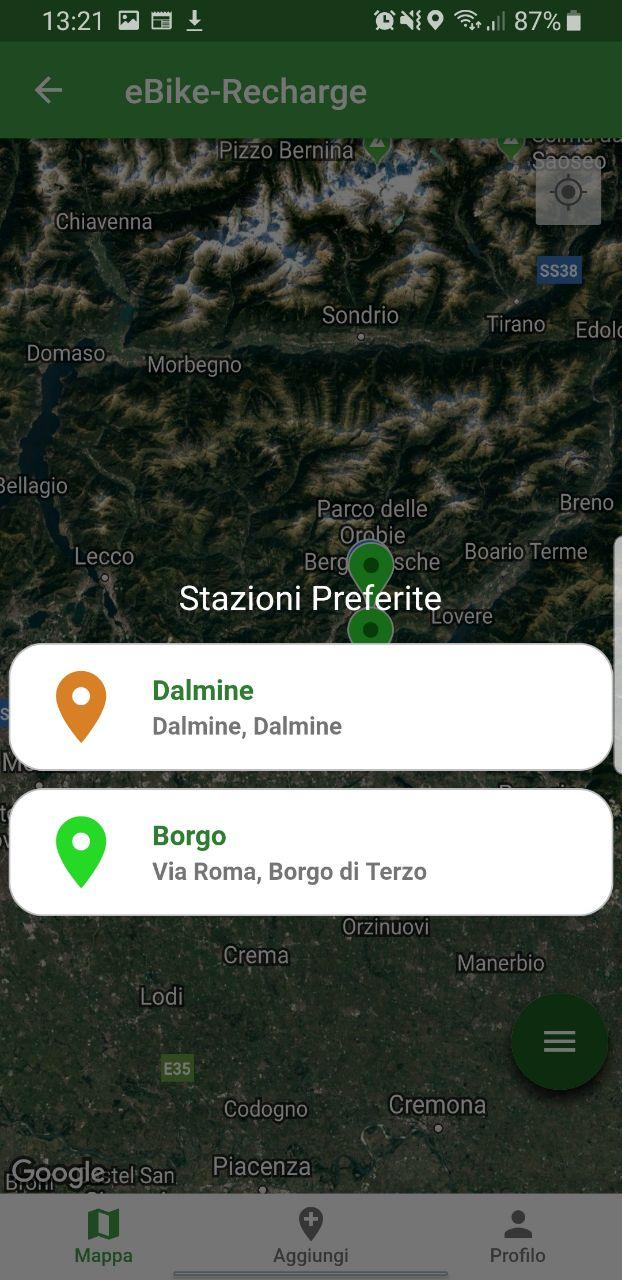
\includegraphics[width=\linewidth, height=9cm]{MapFunFavourite.jpg}
        \caption{Preferiti}
    \end{subfigure}
    \begin{subfigure}{0.3\linewidth}
        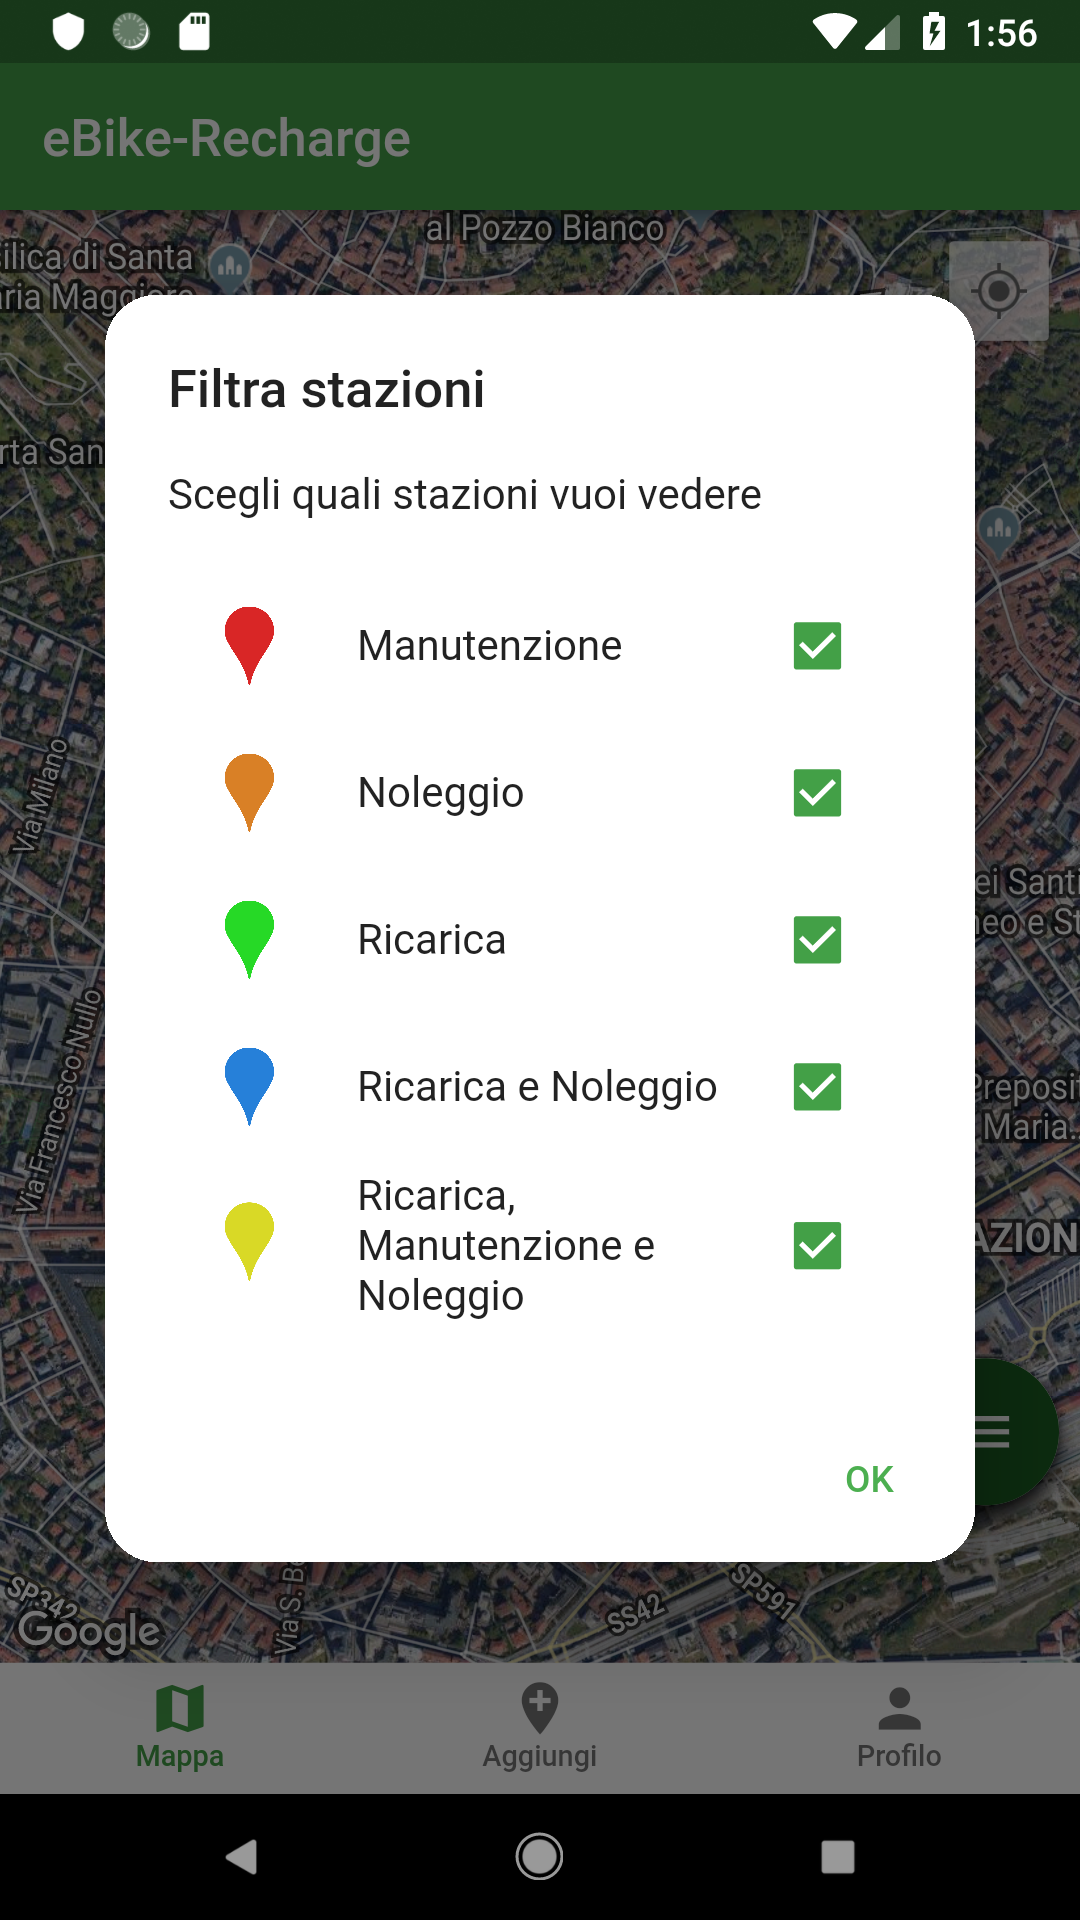
\includegraphics[width=\linewidth, height=9cm]{MapFunFilter.png}
        \caption{Filtro e Legenda}
        \label{filtro}
    \end{subfigure}
    \begin{subfigure}{0.3\linewidth}
        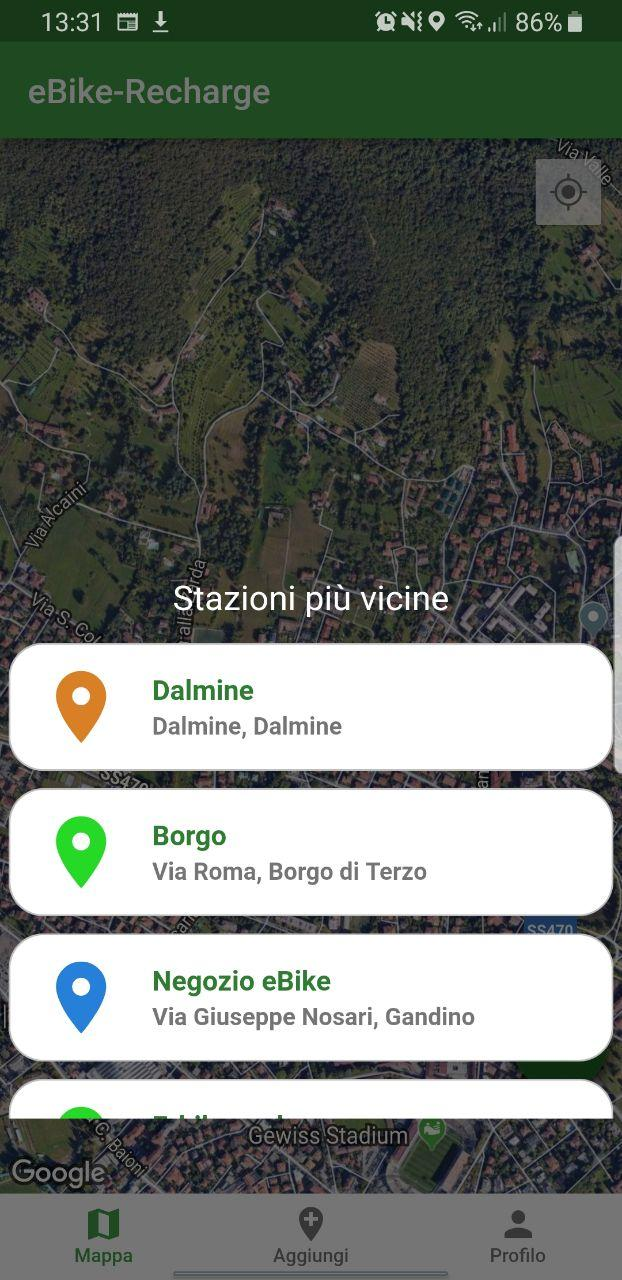
\includegraphics[width=\linewidth, height=9cm]{MapFunNearest.jpg}
        \caption{Stazioni più vicine}
    \end{subfigure}
    \caption{}
\end{figure}

L'ultimo pulsante è accompagnato da un'icona rappresentante una lente di
ingrandimento, simbolo universale di ricerca. Premendolo, in alto sullo schermo
appare un TextField con impresso la frase "Cerca Indirizzo". L'utente è quindi
invitato a digitare la via o la località che desidera vedere. Mentre si forma la
scritta, grazie al servizio API Google Places l'app è in grado di mostrare
diverse Card a schermo con suggerimenti, fungendo quindi da auto-completamento.
Se l'utente clicca su una di queste sezioni viene richiamata la stessa funzione
delle Card prima mostrata: la mappa cambia centro e porta l'utente nella via
desiderata. Questo servizio costa una frazione di centesimo per ogni singola
chiamata alla funzione di auto-completamento. Si è quindi deciso di introdurre
un limite mensile al numero di volte che l'app può far uso di questa API, in
corrispondenza del numero massimo di chiamate che si possono fare senza dover
pagare direttamente Google.
\begin{figure}[!h]
    \centering
    \begin{subfigure}{0.33\linewidth}
        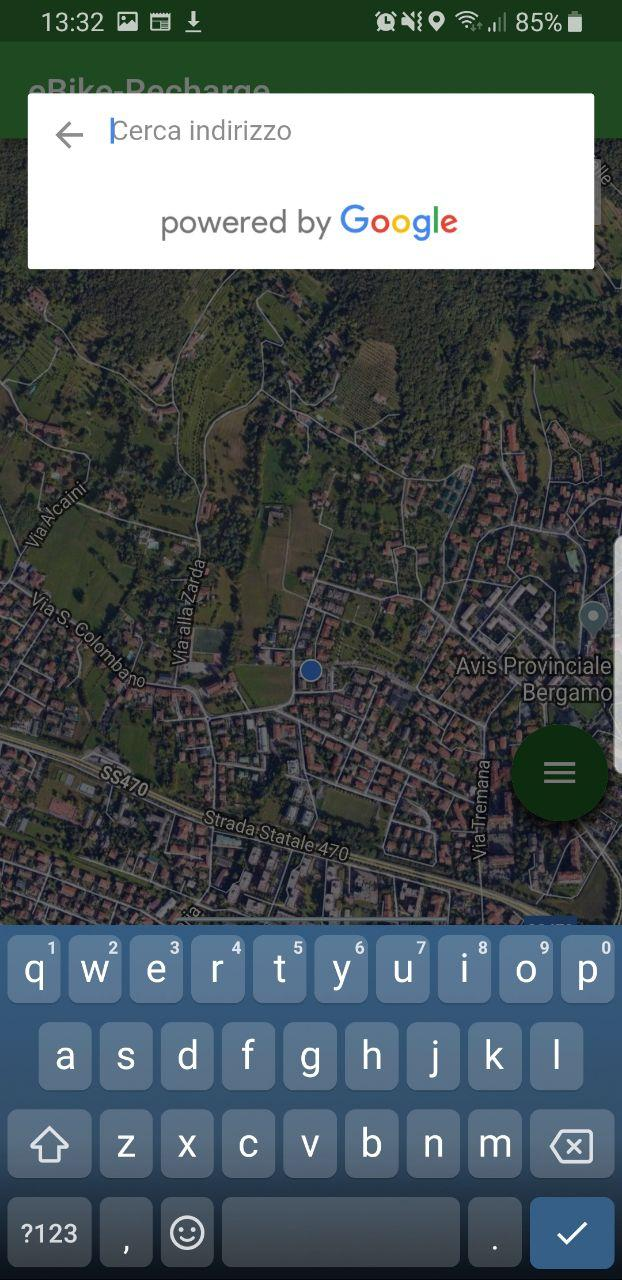
\includegraphics[width=\linewidth, height=9cm]{MapFunSearch1.jpg}
    \end{subfigure}
    \begin{subfigure}{0.33\linewidth}
        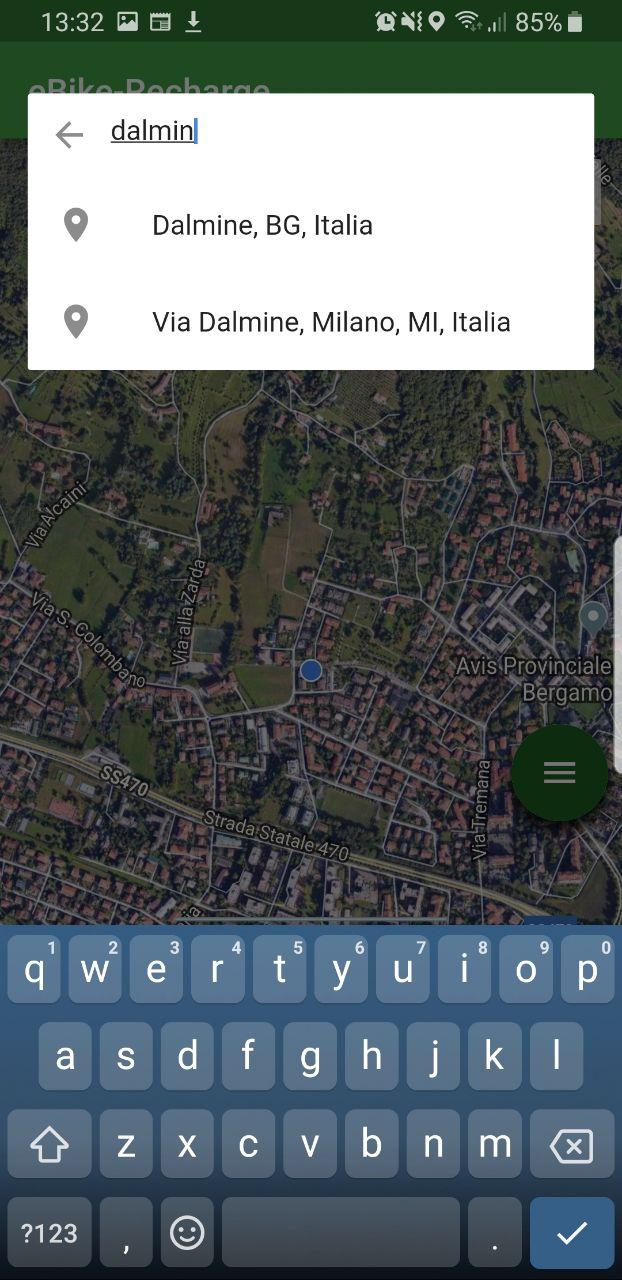
\includegraphics[width=\linewidth, height=9cm]{MapFunSearch2.jpg}
    \end{subfigure}
    \caption{La funzione di ricerca e autocompletamento dell'API Google Places}
\end{figure}

\section{Aggiungere una Stazione}
% \subsection{Aggiungere una Stazione}
Aspetto interessante dell'applicazione è che l'utente, se registrato, ha la
possibilità di inserire lui stesso una nuova stazione e, dopo che essa è stata
approvata dagli amministratori, vederla comparire sulla mappa. Questa funzione è accessibile nella
pagina Aggiungi Stazione, raggiungibile dopo aver premuto l'icona centrale della
BottomNavigationBar. 
\begin{figure}[!h]
    \centering
    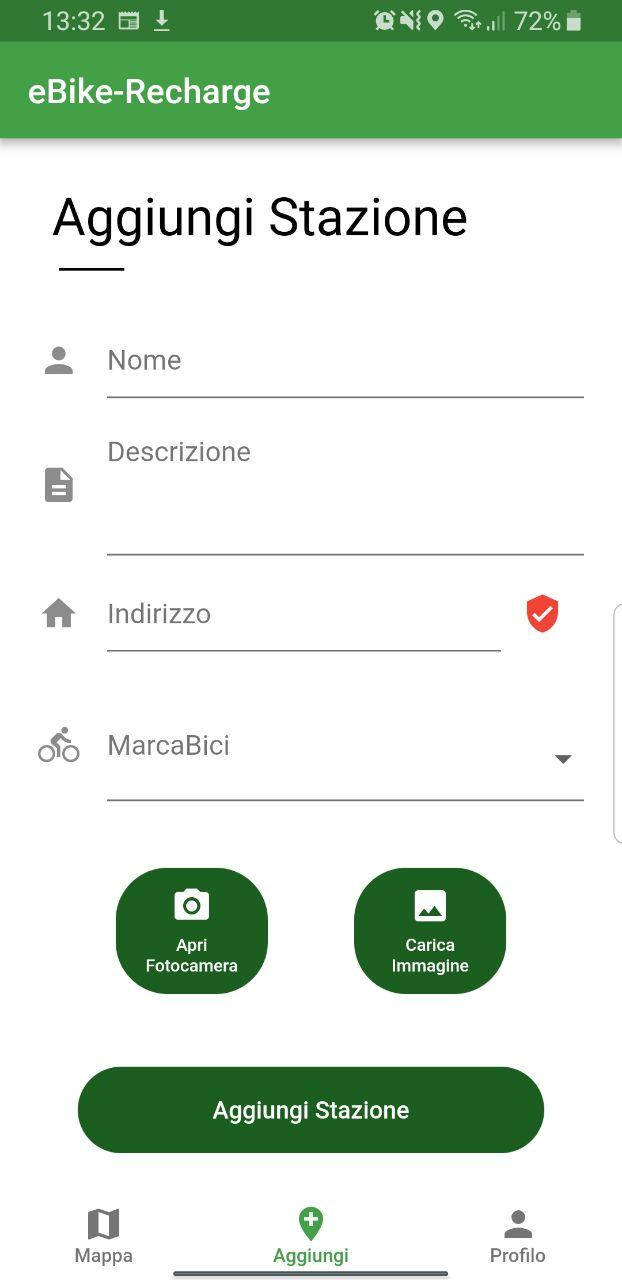
\includegraphics[width=0.33\linewidth,height=9cm]{AddStation1.jpg}
    \caption{Pagina Aggiungi Stazione}
    \label{addStation1}
\end{figure}
La pagina si presenta come in figura \ref{addStation1}. Ogni riga fa parte
dell'unica grande Form che contiene tutte le TextFormField. Ognuna di queste è
formata da un titolo stampato che indica quale dato inserire e che scompare non
appena inizia la digitazione dell'utente in quel particolare campo. 
Il quarto campo è in realtà un menù a tendina e presenta tutte le tipologie di
stazione, raffigurate in figura \ref{addStation4}.
\begin{figure}[!h]
    \centering
    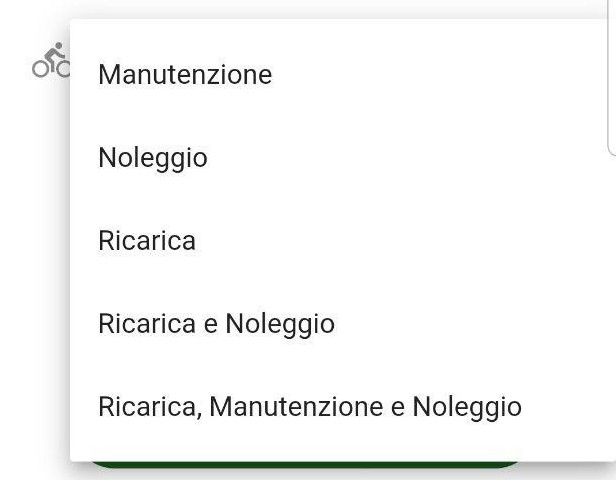
\includegraphics[width=0.33\linewidth]{AddStation4.jpg}
    \caption{Menù a tendina con le tipologie di stazioni}
    \label{addStation4}
\end{figure}

Aver
inserito i componenti all'interno di una Form facilita notevolmente i controlli
per l'integrità dei dati. Infatti, se l'utilizzatore preme il tasto
\textit{Aggiungi Stazione} prima che abbia inserito i dati obbligatori (tutti
fuorchè la descrizione) si avrà la situazione mostrata in figura \ref{addStation2}.
\begin{figure}[!h]
    \centering
    \begin{subfigure}{0.36\linewidth}
        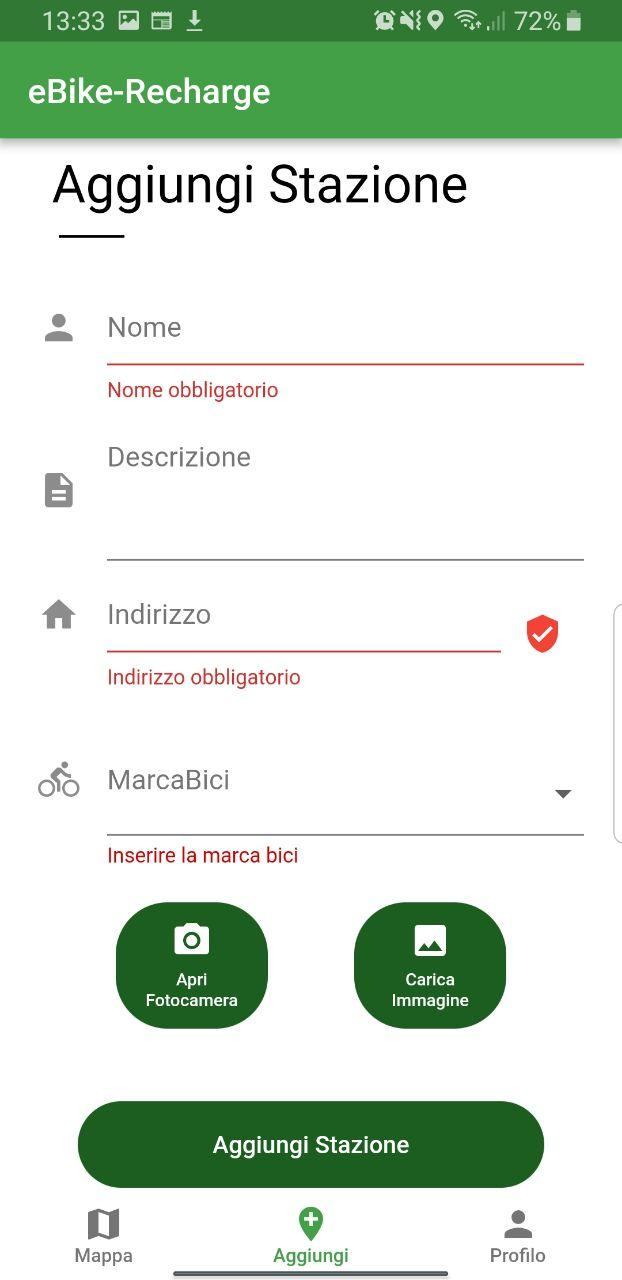
\includegraphics[width=\linewidth,height=10cm]{AddStation2.jpg}
    \end{subfigure}
    \begin{subfigure}{0.36\linewidth}
        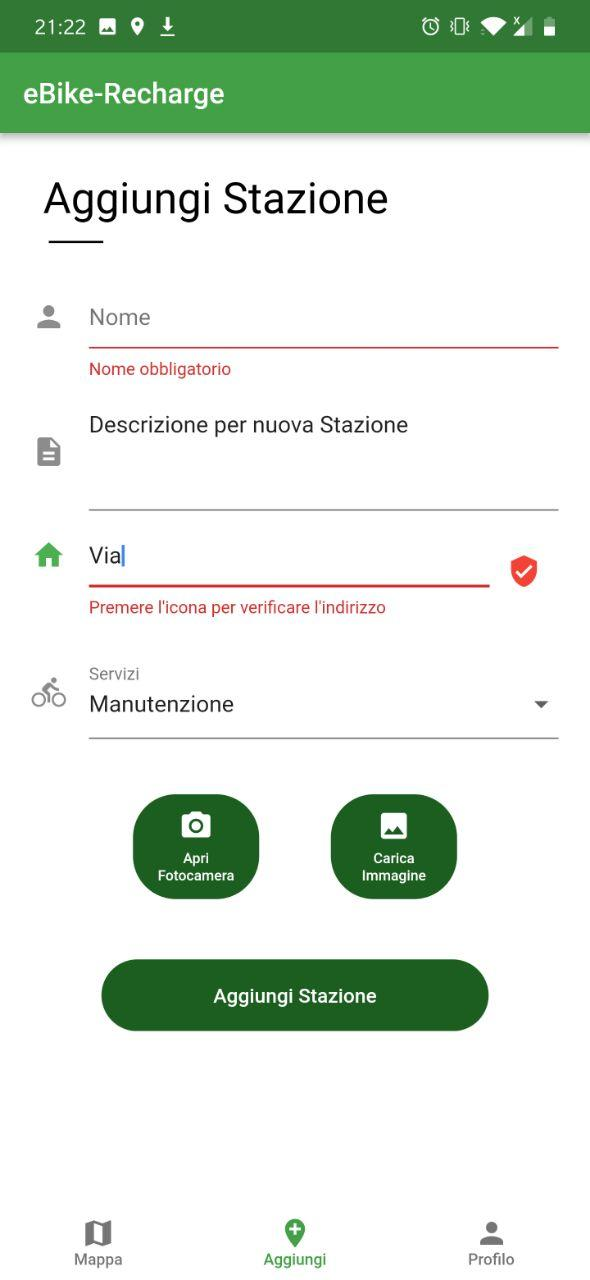
\includegraphics[width=\linewidth,height=10cm]{AddStation3.jpg}
    \end{subfigure}
    \caption{Poichè la funzione onSubmit ha restituito False in almeno un campo,
    lo stato della Form è in Errore, anche se basta cominciare a scrivere
    per cambiarne lo stato.}
    \label{addStation2}
\end{figure}
Sotto tutti i campi in cui non è stato inserito nessun dato, si mostrerà a
schermo una scritta di colore rosso indicante il motivo dell'errore. Questo
accade perchè quando si preme il pulsante viene richiamata la funzione
\textit{onSubmit} che richiama tutte le funzioni dallo stesso nome all'interno
di tutte le TextFormField. Ognuna di queste funzioni deve restituire un tipo di
dato booleano
True o False. Se anche un solo campo restituisce False, tutto lo stato della
Form è considerabile in stato di Errore. Se invece tutti i campi restituiscono
True ecco che allora il controllo è superato e si inserisce la stazione dopo
l'aver confermato la propria scelta. \\
Si  noti come nel campo in cui bisogna indicare l'indirizzo della stazione siano
presenti due diversi tipi di errore: il primo si manifesta nel momento in cui il
campo è vuoto e non ha alcuna parola al suo interno, il secondo quando si
comincia sì a scrivere ma non si ha ancora premuto l'icona rossa a lato, che
serve per cercare esattamente l'indirizzo fornito e tradurlo in coordinate
geografiche (latitudine e longitudine). Quando questo accade l'icona diventa di
colore azzurro (fig. \ref{addStation6}) e la funzione onSubmit di quel particolare campo
restituisce True.
\begin{figure}[!h]
    \centering
    
\includegraphics[width=0.53\linewidth]{AddStation6.jpg}
    \caption{Indirizzo verificato e tradotto in latitudine e longitudine}
    \label{addStation6}
\end{figure}  
\\
Sotto i quattro campi sono presenti due pulsanti con le scritte \textit{Apri
Fotocamera} e \textit{Carica Immagine} (fig. \ref{addStation5}). Come ben indicato dal nome, questi due
Container sono stati codificati per diventare pulsanti che permettono
all'utente di indicare un'immagine catturata dalla propria fotocamera o
all'interno 
della galleria. Ovviamente al primo accesso l'app chiede il permesso
all'utilizzatore di accedere sia alla fotocamera che alle immagini presenti nello storage
interno del proprio device. Caricata l'immagine, è possibile vedere la propria
scelta all'interno della pagina e premendo la \textit{X} rossa che compare a schermo,
eliminarla e prenderne in considerazione altre.
\begin{figure}
    \centering
    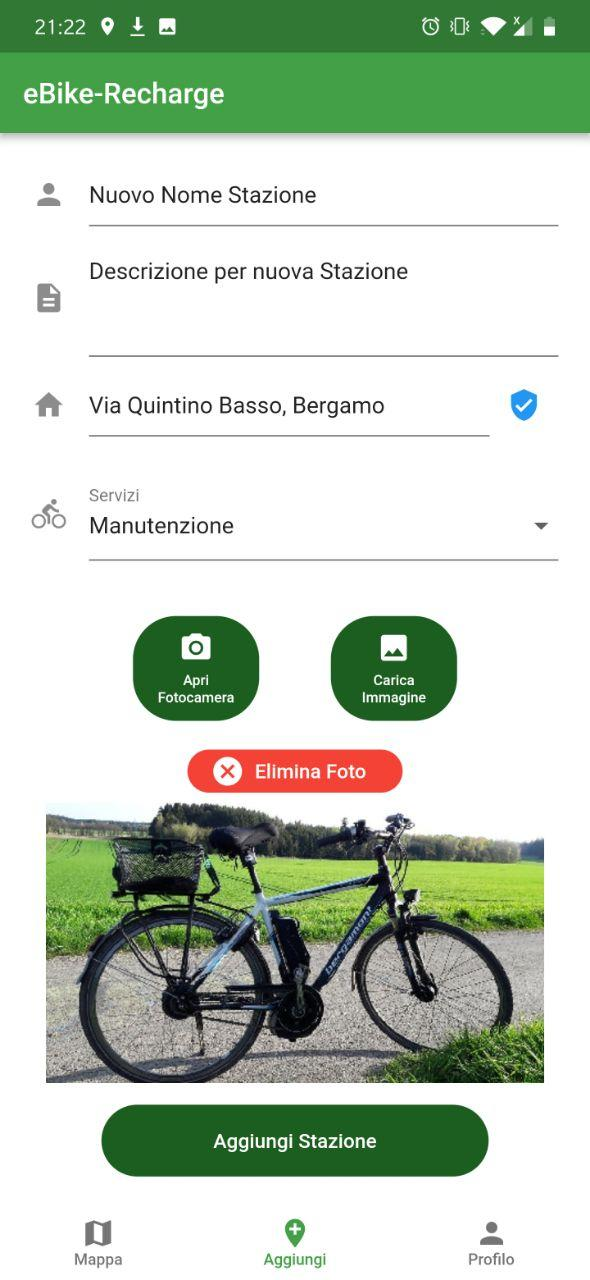
\includegraphics[width=0.33\linewidth]{AddStation5.jpg}
    \caption{Pagina con immagine caricata dalla galleria}
    \label{addStation5}
\end{figure}
\begin{figure}[!h]
    \centering
    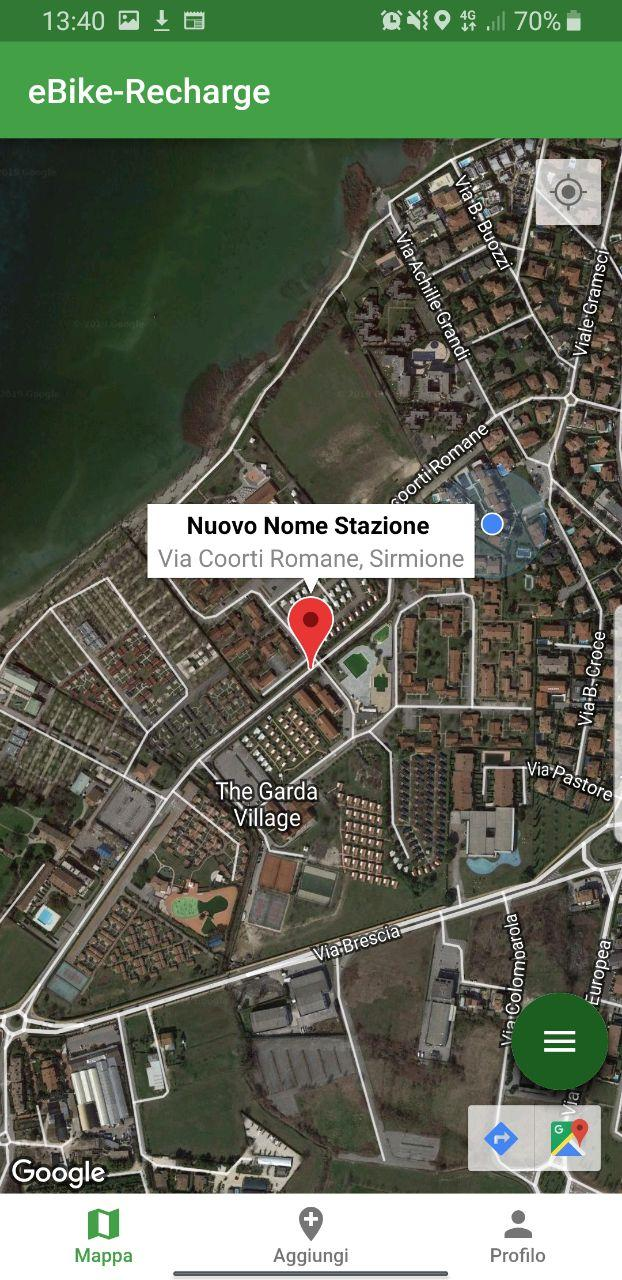
\includegraphics[width=0.33\linewidth]{AddStation7.jpg}
    \caption{Nuova stazione inserita che ha superato tutti i controlli}
    \label{addStation7}
\end{figure}
Terminato il passo precedente e dopo aver confermato che tutti i dati inseriti
abbiano superato il controllo della Form, la stazione è aggiunta nel database
dell'applicazione. Per prevenire che utenti malintenzionati inseriscano stazioni
che in realtà non esistono o inseriscano dati non coerenti, ogni stazione appena
aggiunta presenta un campo di flag impostato a False. Sarà poi compito del gestore
dell'app che periodicamente controlla le nuove aggiunte verificare la
veridicità dei dati inseriti e impostare a True il campo flag. Dopo questa
operazione la stazione diventa visibile per tutti gli utenti come in figura
\ref{addStation7}.

\section{Codifica}
Data la quantità di codice che è stato sviluppato per fornire la mappa di tutte
le sue funzionalità, nel seguito verranno solo indicati gli aspetti principali.
\begin{minted}[	frame=lines, framesep=2mm, baselinestretch=1.2,
    fontsize=\footnotesize, linenos 	] {python}
GoogleMap(
    minMaxZoomPreference: MinMaxZoomPreference(5.0, 20.0),
    markers: _markers,
    compassEnabled: true,
    mapType: _tipoMappa,
    myLocationEnabled: true,
    cameraTargetBounds: CameraTargetBounds(LatLngBounds(
        southwest: LatLng(44.4264, 8.91519),
        northeast: LatLng(46.0693, 13.23715))),
    initialCameraPosition: CameraPosition(
        zoom: 15.0,
        target: LatLng(
            currentLocation.latitude, currentLocation.longitude),
    ),
    onMapCreated: onMapCreated,
),
\end{minted}
Nel frammento di codice della pagina precedente si può notare come la mappa venga creata mediante
l'oggetto \verb|GoogleMap|, presente all'interno del pacchetto
\textit{google\_maps\_flutter}. Il suo costruttore ha a disposizione numerosi
argomenti per personalizzare ciò che si vuole visualizzare. Nel caso in cui
alcuni attributi non vengano indicati, l'oggetto provvederà a definirli con casi
standard (come la tipologia Normale per il tipo di mappa). Seguendo la figura, è
possibile indicare il minimo e il massimo zoom applicabile alla schermata
(ottenibile avvicinando o allontanando le dita), indicare i marker, cioè i punti
di interesse (ognuno con il proprio colore, titolo e descrizione), e permettere
o meno la rotazione della visuale. Si può poi indicare il tipo di mappa,
visualizzare a schermo la propria posizione e introdurre dei limiti invalicabili
indicati tramite coordinate geografiche. In particolare, data la natura
dell'app, si è scelto di porre come vincolo a SudOvest la posizione della città
di Genova, e come vincolo a NordEst la città di Udine. Infine è possibile
indicare la posizione iniziale della \textit{camera} (visuale) della
mappa e indicare quale meteodo debba essere eseguito nel momento in cui il
widget è stato creato e caricato correttamente. Nello specifico, il metodo
onMapCreated del progetto consiste nell'assegnare alla mappa un controller di
tipo \verb|GoogleMapController|. Questo permette di spostare la visuale e di
aggiungere ed eliminare marker dalla mappa, creando un vero e proprio oggetto in
grado di controllare il widget. \\
\begin{minted}[	frame=lines, framesep=2mm, baselinestretch=1.2,
    fontsize=\footnotesize, linenos 	] {python}
void zoomInMarker(Stazione stazione) {
    mapController.animateCamera(CameraUpdate.newCameraPosition(CameraPosition(
        target: LatLng(
            stazione.coords.latitude,
            stazione.coords.longitude),
        zoom: 14.0,
        bearing: 90.0,
        tilt: 45.0)));
}
\end{minted} 
Il codice sopra riportato mostra il metodo \verb|zoomInMarker| che aumenta lo zoom della visuale a
seguito della pressione da parte dell'utente del titolo di uno specifico marker,
il tutto con un gradevole effetto dovuto alla rotazione. Questo è reso possibile
dall'oggetto mapController che, tramite il metodo \verb|animateCamera| (il quale prende
in input un oggetto di tipo \verb|CameraUpdate|), porta la visuale al nuovo
target specificato, sempre usando la latitudine e la longitudine. \\
Si noti infine il codice nella pagina successiva che mostra la funzione
\verb|searchAndNavigate|. Come indica il nome, questa porzione di codice prende
in input una stringa di testo, cioè l'indirizzo cercato dall'utente, e allo
stesso modo di prima porta la visuale della mappa nella località indicata
convertendo i caratteri in coordinate geografiche. Questo processo è dovuto
al metodo \verb|Geolocator().placemarkFromAddress()| ottenibile dal
pacchetto \textit{geolocator}. Il risultato dell'operazione è di tipo Future e
per questo è utilizzabile solo con un metodo then (chiamata asincrona). L'output
è dunque un vettore contenente per ogni elemento una località con diversi
attributi (nella figura si possono notare i campi name, locality e position, che
a sua volta possiede latitude e longitude). L'ultimo passaggio è il medesimo
visto nel caso precedente spostando la visuale con l'oggetto mapController. \\ \\
\begin{minted}[	frame=lines, framesep=2mm, baselinestretch=1.2,
    fontsize=\footnotesize, linenos 	] {python}
void searchAndNavigate(String testo) {
    Geolocator().placemarkFromAddress(testo).then((result) {
        searchController.text = result[0].name + ', ' + result[0].locality;
        mapController.animateCamera(CameraUpdate.newCameraPosition(CameraPosition(
        target:
            LatLng(result[0].position.latitude, result[0].position.longitude),
        zoom: 15.0,
        )));
    });
}
\end{minted}